\documentclass[a4paper]{llncs}
\usepackage[utf8]{inputenc}
\usepackage{times,verbatim} % Please do not comment this
\usepackage{graphicx}
\graphicspath{ {images/} }

\begin{document}

	\pagestyle{empty}

	\mainmatter

	\title{Cybersecurity and honeypots: experience in a scientific network infrastructure} 

	\titlerunning{Cybersecurity and honeypots: experience in a scientific network
infrastructure}

	\author{Juan Luis Martin Acal \and Gustavo Romero López \and Pablo Palacín Gómez \and Pablo García Sánchez \and Juan Julián Merelo Guervós \and Pedro A. Castillo Valdivieso }

	\authorrunning{Juan Luis Martin Acal}

	\institute{Departamento de Arquitectura y Tecnología de Computadores.\\ ETSIIT - CITIC. University of Granada, Spain\\
	\email{jlmacal@correo.ugr.es}\\
	\email{\{gustavo, pablo, pablogarcia, jmerelo, pacv\}@ugr.es}\\
	}

	\maketitle

\begin{abstract}
When dealing with security concerns in the use of network infrastructures a good balance between security concerns and the right to privacy should be maintained. This is very important in scientific networks, because they were created with an open and decentralized philosophy, in favor of the transmission of knowledge, when security was not a essential topic.
Although private and scientific information have an enormous value for an attacker, the user privacy for legal and ethical reasons must be respected. Thus, passive detection methods in cybersecurity such as honeypots are a good strategy to achieve this balance between security and privacy in the defense plan of a scientific network. In this paper we present the practical case of the University of Granada in the application of honeypots for the detection and study of intrusions, which avoid intrusive techniques such as the direct analysis of the traffic through networking devices.
\end{abstract}


\section{Introduction}
From the earliest days of computer networks, these have been experiencing continued growth in number of attacks \cite{esset-tendencias,cni-ccn-tendencias-2014,cni-ccn-tendencias-2015}. The complexity of these attacks against the information and resources in the networks has also increased. This escalation is motivated by economic, politic or military interests or by the same entities interested in exercise a bigger control over communication freedom in the Internet \cite{cni-ccn-tendencias-2015,cisco-2014}.

Although private and scientific information have an enormous value for an attacker, the user privacy for legal and ethical reasons must be respected by the Chief Security Officer (CSO). Scientific networks are a special and interesting case; in one hand there is a strong demand of security in the network and the resources and services which are listening. On the other hand, the end users demand privacy in his network traffic covered by the law. But classic Scientific networks were not designed thinking in security concerns \cite{iris-proyecto}. In contrast to the corporate networks, which usually have grown from the intranet to the Internet, and which have the most of hosts behind the demilitarized zone (DMZ), the scientist networks were born with an open philosophy without focusing on security \cite{iris-proyecto}. Only technical requirements such as the limited number of public IP address forced it to expand private services to the intranet. The information related to research, patents, computer and human resources is a juicy target for hostile agents. Also, the big size of the DMZ makes it prone to a massive attack and increases the possibility of finding a security breach or hide advanced vectors of attack. In this scenario the passive sensors have an important role in the detection and protection against cyber-attacks.

In this paper is presented the deployed of a security system in the University of Granada based in passive sensors in order to avoid intrusive techniques such as the direct analysis of the traffic through networking devices, and also it is exposed some test with the finality of complementing the manual tracking of incidents.

The rest of the paper is organized as follows: Section \ref{sec:deployment} the characteristic of the passive sensor and the infrastructure used are expected. In the section \ref{sec:analysis}, the analysis of the registered data is presented. A critical analysis of the strong and weak points for the infrastructure exposed is made. Section \ref{sec:Strengths&Weaknesses} explains some experiments with machine learning based in Kohonen's self-organizing maps (SOM) \cite{kohonen-1990} in order to improve the data analysis. Finally, we present concluding remarks and suggestions for future study.


\section{Deployment of a Security System Based in Honeypots}
\label{sec:deployment}
This section describes the deploy of the system responsible for detecting the malicious activity in the network infrastructure and its components. Also, the elements and methods to use will be described.

\subsection{Honeypots}
A honeypot is a computer trap that exposes itself as bait. While the honeypot is scanned, probed or compromised by a cyber attack, it is collecting information about the malicious activity. The deception techniques have been present in tracking of security incidents \cite{Cheswick92anevening}, even before its use in security software \cite{DTK,RoleOfDeception}. Honeypots were introduced in the cyber security investigation world by {\it``The Honeynet Project"} a nonprofit research group in 1999, in their series of papers {\it``Know Your Enemies"} \cite{KnowYourEnemies}. There are different classification characteristics such as interaction, distribution appearance or role in multi-tier architecture \cite{Seifert06taxonomyof}. The interaction is the degree of fidelity in the response of the trap. The distribution appearance describes whether the honeypot system appears to be confined to one system or multiple systems. Role, describes in what {\it role} acts within a multi-level architecture and can be server or client.

There is not an ideal configuration of features, or distribution of them inside de network, as there exist a huge effect on the nature of the threats and in the infrastructure to protect. For example in software development environments, high interaction are used for testing new products with {\it fuzzers} or another type of Penetration Testing (informally called {\it pentesting}) tool \cite{fuzzingforsec} in order to discover potential vulnerabilities. On the other hand, low interaction honeypots are used like intrusion detection systems, warning about activity of scans or jumping attempts from compromised internal hosts within production environments. Both share a common point: they are not intrusive with the network traffic.The architecture in our system is divided in two fronts:
\begin{itemize}
	\item The management front has the task to help the operator to manage all the information related to security incidents.
	\item The detection front is based on honeypots of medium and low interaction with stand-alone distribution appearance and server role.
\end{itemize}

\subsection{Deployment}
The sensors were deployed in different production subnets and each one included honeypot software. Specifically Dionaea \cite{dionaea} and Kippo \cite{kippo}, which are low and medium interaction honeypot respectively. Each sensor has local databases with the purpose of saving efficiently the information about attacks, while is waiting to dump the data in the collector. This is done in order to keep the information duplicated and not to increase the network traffic in case of massive scans or attacks. Between two consecutives data dumps to the centralized data collector, the sensors send incidents by mean of the Linux client of the messaging software ``Telegram'' \cite{telegram-messenger} to the operator, in time-lapses lower than 5 minutes. The collector is a corporate database that feeds the incidents management system, and it is the source of the analyzed data.

\section{Data analysis}
\label{sec:analysis}
This section is details the analysis of the information gathered and the behavior of detected cyber threats. We explain how this information shows the stages of the complex threats involved in multivector attacks, and is discovered the finality behind of advanced threats.

For three years each sensor collected information of about half a million of connections. The analysis of this high amount of information has provided the next facts:
\begin{itemize}
	\item External attacks are more frequent than internal attacks.
	\item In one hand the most frequent type of external attacks was weak credentials disclosure. On the other hand, the most frequent type of internal attack is the attempt of malicious software ({\it malware}) propagation.
	\item The incident tracking shows how countries outside NATO are the most active in the process of scanning and searching for vulnerabilities; but curiously most of the intrusions come from NATO member or member candidate countries. It is important to note that this data depends on the geolocation where was taken and the relationship with other countries \cite{wiki-cyberwarfare-china,wiki-cyberwarfare-eeuu}.
\end{itemize}

\begin{figure}[h]
	\centering{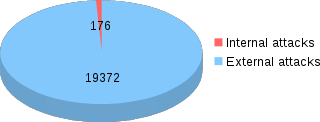
\includegraphics[width=0.49\textwidth,keepaspectratio]{dionaeaInternalExternal.png}}
	\label{fig:intvsextDionaea}
	\centering{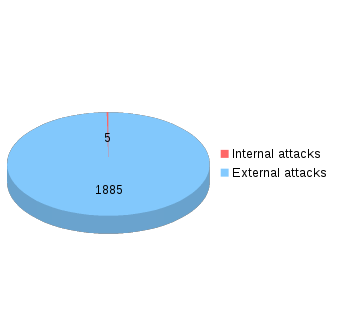
\includegraphics[width=0.49\textwidth,keepaspectratio]{kippoInternalExternal.png}}
	\label{fig:intvsextKippo}
	\caption{On the left, the number of IP involved in external attacks versus internal attacks detected by Dionaea. On the right, the number of IP involved in external attacks versus internal attacks detected by Kippo.}
\end{figure}

Collected data shows how external attacks are the most frequent source of attacks. This matches with studies of big security IT enterprises \cite{verizon-2015}. Several connections were obtained, some of them from scans to the network infrastructure and others looking for exploiting vulnerabilities or services without strong credentials. Respecting the latter, it is necessary to emphasize those that showed a more advanced level in the process of intrusion because were linked to Advance persistent threats (APT). One of the greatest dangers for IT infrastructures of governments, public administrations and companies are advanced persistence threats. A cyber threat is persistent if it is continuous in time and establishes monitoring and control mechanisms with a hostile agent. It is advanced if uses mechanisms in order to hide its activity in the system. Usually APT are related with cyberspying and elite groups of cybercrime and they are attacks directed against a specific infrastructure. For this reason, it is a priority to detect and study them.

The attempts of malware propagation usually belong to advanced and persistent threats and come included in multivector attacks. A attack is multivector whether it exploits multiple vulnerabilities in order to reach the intrusion and compromised goals. When a Windows host belonging to the infrastructure was compromised by a USB drive, after had communicated its incorporation to the command and control server of the netbot, it started to scan its neighbors within the subnet. Then, it established connections with the sensors that  emulated the ms08-067 \cite{ms08067} vulnerability. After this, it commanded to the honeypot software download the binary of trojan from a external web servers. This strategy avoided that firewalls blocked external infections to internal hosts through Server Message Block protocol (SMB) services. Finally, the infected host, would tried to spread the infection, scanning and attacking others subnets, this process is named {\it jumping}. In our system, this last stage was prevented by the low interaction characteristic.

\begin{figure}[h]
	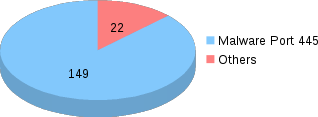
\includegraphics[width=0.5\textwidth]{internalTypes.png}
	\centering
	\label{fig:internalTypes}
	\caption{The malware was main source of internal attacks, and shows a advanced behavior involved in multivector attacks.}
\end{figure}

It is quite difficult to follow the clue for rebuilding of multivector attack. Usually the exploitation of SSH or MySQL weak credentials is the first step to gain the control, or access to data, in the emulated server. But only a very reduced part shows a clever behavior behind the attack. Between hundred of thousand of connections only a few ones shows access to the fake information such as fake passwords. Then, intelligent attacker tried to use this information against other services with the purpose of  ``jumping'' inside them. A bit more frequent is the attempt to privilege elevation. But the common behavior is to use the basic vulnerability in order to use his network and computational resources as soon as possible. This resources were collected for using in tasks like miner Litecoin \cite{litecoin}, increase the number of nodes for other network scans, for a future deny of service (DoS) attack or for using the compromised host like a anonymous proxy.

When we rebuild the trace of the attack, the first advanced behavior that we find is the use of different hosts for scanning the infrastructure and change to others hosts for the exploitation. The attack starts to scan subnets usually from countries without collaborations accord, in our case China but finally the exploitation is from Europe or United States.

\section{Strengths and Weaknesses of Honeypots}
\label{sec:Strengths&Weaknesses}
The strengths of honeypots and the deployed system are:
\begin{itemize}
	\item It was not intrusive with network traffic, remained the privacy of infrastructure users. This is an important point because any try to catch indirect traffic network could be seen as a threat by other users and an infringement of the using conditions of the network and legality.
	\item The computational and economic resources needed for passive detection are lower because only the traffic belonging to a potential cyber threat are available. This an alternative approach to other solutions, more expensive, like intrusion detection systems based in hardware.
	\item Cyber threats, such as advanced malware, uses ciphered communications in order to dodge detection systems in the network layer. The only way to catch information is from inside of the compromised node. This is essential to analyze how persistence cyber threats monitor the compromised host and what information is sent outside, to the command and control network.
\end{itemize}

In another hand the weakness of honeypots and the deployed system are:
\begin{itemize}
	\item There are many cyber threats focused in the network layer, usually related with deny of services and spoofing. This information is very valuable because this kind of attack are a very important element not only in simple vector attacks, in multivector advanced and persistent attacks too. Honeypots only fetch information from the application layer so they lose essential information for reconstruction of complex attacks.
	\item The use of passive sensors in a security system must be planned with some extra considerations respect to the use of active methods of detection. Those considerations cover strategies of deception and hiding of the sensors and politics of migrations in the infrastructure for avoiding it's location.
	\begin{itemize}
		\item Like others deception tools, honeypots must show as interesting targets for a attacker and avoid them to be easily recognizable by fingerprint techniques. Default installations and configurations in low an medium interaction honeypot are easily detected by a human attacker or an intelligent threat like advanced malware.
		\item When attacker has knowledge of the infrastructure, honeypots are easily dodged so must be deployed together with politics of use, like change its subnets or IP every so often.
		\item High interaction honeypots are dangerous in production environments because the monitored sensor is completely real and all his potential in order to attack its periphery. Usually they are deploying in isolated subnets with outgoing traffic strongly restricted in company of others honeypots, that configuration is called honeynet.
	\end{itemize}
\end{itemize}

\section{Experiments with S.O.M}
\label{sec:Improve}
In this section, we expose an experiment with Self-Organizing Maps so as to classify information and we comment some interesting results.

In order to classify the information of detected attacks, we apply the classification method that is described in \cite{panda-2009}, in two subsets of data. The first advantage is the simplification of the collected information derived from the dimensional reduction intrinsic to the method. The attacks are organized in 2D clusters.  This allows identify some interesting characteristics. As the first result, it can be seen The first thing that drawing our attention is how the attacks to HTTP, Microsoft SQL Server (MSSQL) and Session Initiation Protocol (SIP) are concentrated in areas better defined. It is because the cyberthreats showed less variability in their dimensional components. This can be explained by the nature of the connections of the attacks and the characteristics of the software used. A sweep scan to search for services in parallel with tools such as Nmap \cite{nmap} or malware with a very aggressive behavior, have a great variability in the component {\it"source port"}. On the other hand when the connection comes from targeted attacks or advanced malware, the behavior observed is discrete so as to avoid intrusion detection systems, variability is lower.

\begin{figure}[h]
	\centering{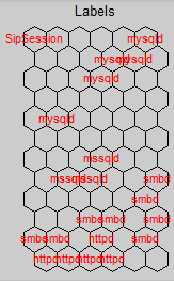
\includegraphics[height=0.333\textheight,keepaspectratio]{subset1.png}}
	\label{fig:intvsextDionaea}
	\centering{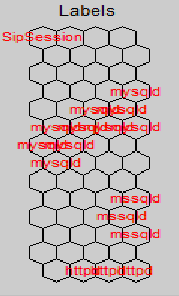
\includegraphics[height=0.333\textheight,keepaspectratio]{subset2.png}}
	\label{fig:intvsextKippo}
	\caption{On the left, the first subset of gathered attacks. On the right, the second subset of gathered attacks. Some services shows clusters more dispersed than other.}
\end{figure}

Finally, information about fake advanced attack was injected in the first subset and the union of the previous subsets in a third subset was built. The information from both honeypots is arranged around the second diagonal. In the lower right area a cluster with connection attempts to MySQL service number displayed readily inverted port. Changing the default port number is a common practice to hide services. Port scannings with reverse numbering or multiple of the original denotes an intelligent behavior. S.O.M allow to obtain visual information to study it easily looking for  anomalies, candidates to attacks, with a intelligent behavior.

\begin{figure}[h]
	\centering{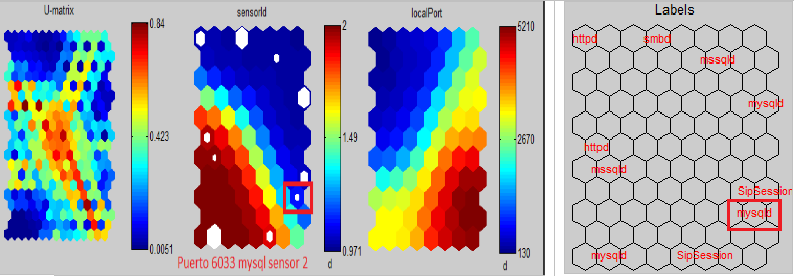
\includegraphics[width=12cm,height=6cm,keepaspectratio]{subset3.png}}
	\label{fig:internalTypes}
	\caption{Union between firs and second subset. The information is auto organized around the second diagonal and it was detected a fake attack to a hidden MySQL port such as a individual cluster.}
\end{figure}

\section{Conclusion and Future Works}
\label{sec:conclusion&future}
We have exposed how is possible a security system based in passive sensors. The range of detected attacks goes from elementary scans, to attempts of intrusions and malware injections. Although it is possible to identify and track manually APT, this is not efficient, and easily APT can pass unnoticed. Another problem is that the caught information with low interaction honeypots, it is restricted to the application layer. Classification methods initially discover information hidden by the large volume of data. 
For this reason, it is proposed for future works the analysis of data from different sources in hybrid architectures, with different levels of interactions and the comparison. As well as the use of different machine learning methods, supervised or unsupervised, in order to improve the detection of cyber threats.

\bibliographystyle{splncs03}
\bibliography{articuloHoneypot}

\end{document}
